\documentclass[tikz,border=7pt]{standalone}
\usepackage{amsmath}
\usetikzlibrary{arrows.meta,positioning,calc}

\tikzset{
  comp/.style={draw,rectangle,minimum width=26mm,minimum height=12mm,align=center},
  signal/.style={-{Latex[length=2.2mm]},thick}
}

\begin{document}
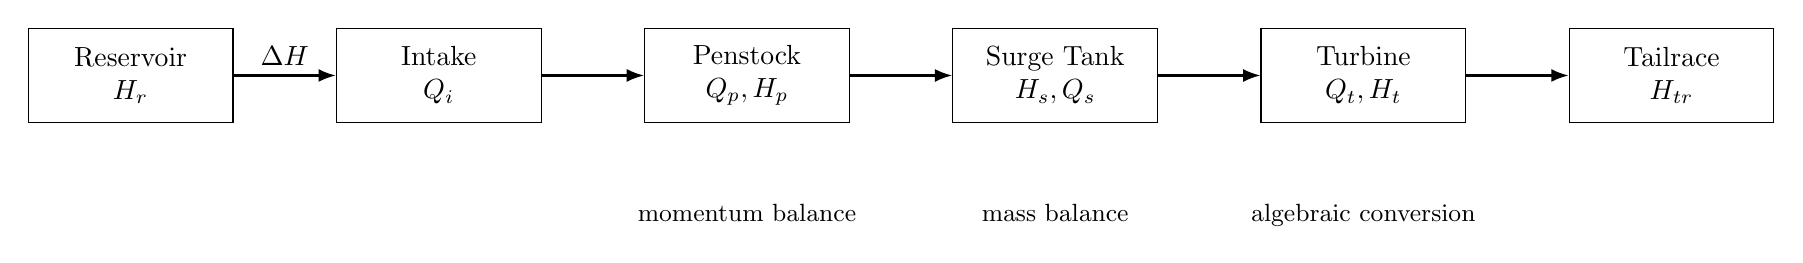
\begin{tikzpicture}[node distance=13mm]

\node[comp] (res) {Reservoir\\$H_r$};
\node[comp, right=of res] (intake) {Intake\\$Q_i$};
\node[comp, right=of intake] (pipe) {Penstock\\$Q_p,H_p$};
\node[comp, right=of pipe] (surge) {Surge Tank\\$H_s,Q_s$};
\node[comp, right=of surge] (turb) {Turbine\\$Q_t,H_t$};
\node[comp, right=of turb] (tail) {Tailrace\\$H_{tr}$};

\draw[signal] (res) -- node[above] {$\Delta H$} (intake);
\draw[signal] (intake) -- (pipe);
\draw[signal] (pipe) -- (surge);
\draw[signal] (surge) -- (turb);
\draw[signal] (turb) -- (tail);

\node[below=9mm of pipe, align=center] {\small momentum balance};
\node[below=9mm of surge, align=center] {\small mass balance};
\node[below=9mm of turb, align=center] {\small algebraic conversion};

\end{tikzpicture}
\end{document}
